\documentclass{article}
\usepackage[utf8]{inputenc}
\textheight = 25cm 
\textwidth = 15cm
\topmargin = -2.5cm 
\oddsidemargin = 1.5cm
\usepackage{float}
\usepackage{graphicx}
\graphicspath{{./images/}}

\usepackage{amsmath}
\usepackage{mathtools, xparse}
\usepackage[shortlabels]{enumitem}
\usepackage[most]{tcolorbox}
\usepackage{adjustbox}
\usepackage{bm} 

\DeclarePairedDelimiter{\norm}{\lVert}{\rVert}

\title{Tarea 8 Mecánica Analítica}
\author{Cerritos Lira Carlos}
\date{6 de Mayo del 2020}

\begin{document}
\maketitle
\section*{Problemas}
\section*{1.-}
\subsection*{6.7)}
En un espectrómetro de masas, se acelera un ion posotivo de una sola carga 
($q=1.602 \times 10^{-19} coloumbs$) por medio de una diferencia de potencial de 
$1000 voltios$. Luego pasa por un campo magnético uniforme en el que $B=0.1weber/m^2$,
y se desvía en una trayectoria circular de $0.182m$ de radio. Determinar:
\begin{enumerate}[a)]
    \item La velocidad del ion.
    \item La masa del ion en kilogramos y unidades de masa atómica.
    \item El número de masa del ion.
\end{enumerate}
\begin{tcolorbox}[breakable]
    \subsubsection*{a)}
    Encontramos la velocidad usando la energía potencial:
    \[ v^2 = \frac{2qV}{m} \]
    encontramos la masa usando el movmiento circular que sigue una vez entra al campo magnético, donde:
    \[ v = \frac{rqB}{m} \]
    juntando ambas obtenemos:
    \[ v = \frac{2V}{rB} = 1.1 \times 10^5 m/seg\]
    \subsubsection*{b)}
    \[ m = \frac{2qV}{v^2} = 2.65 \times 10^{-26}kg = 15.97uma\]
    \subsubsection*{c)}
    \[ A = 15 \]
\end{tcolorbox}

\section*{2.-}
\subsection*{6.9}
En la posición $x=0, y=0$, un cañón tiene un alcance máximo $l_m$. Determinar los dos 
ángulos de elevación para hacer blanco en el punto:
\[ x = l_m/2, \quad y=l_m/4 \]
\begin{tcolorbox}[breakable]
    \[ \theta = 45, 75 \]
\end{tcolorbox}

\section*{3.-}
\subsection*{8.13}
Una cuenta de masa $3m$ puede deslizarse horizontalmente sin rozamiento por un alambre 
como se indica en la figura $8-14$. Unido a la cuerta hay un péndulo doble. Si, en una 
posición cercana a la de su equilibrio, se deja el sistema en libertad, a partir del
reposo, las masas oscilan en el plano de la figura a un lado y al otro de la vertical.
\begin{enumerate}[a)]
    \item Escriba las ecuaciones de Lagrange del movimiento del sistema.
    \item Hállese las aceleraciones cuando los desplazamientos y las aceleraciones son pequeñas.
\end{enumerate}
\begin{figure}[H]
    \centering
    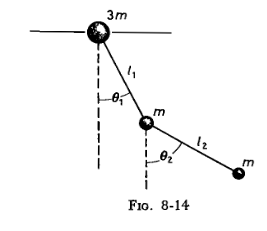
\includegraphics[scale=0.8]{p3_pendulum.png}
\end{figure}
\begin{tcolorbox}[breakable]
    \subsubsection*{a)}
    Sean $x,x_1,x_2$ la posición de las masas, definimos los vectores:
    \begin{align*}
        \bm{e}_{r_1} &= sin\theta_1\bm{i} - cos\theta_1\bm{j} \\
        \bm{e}_{\theta_1} &= cos\theta_1\bm{i} + sin\theta_1\bm{j} 
    \end{align*}
    con ayuda de estos vectores describimos el movimiento:
    \begin{align*}
        \bm{x} &= x\bm{i} \\
        \bm{x}_1 &= \bm{x} + l_1\bm{e}_{r_1} \\
        \bm{x}_2 &= \bm{x}_1 + l_2\bm{e}_{r_2} 
    \end{align*}
    de donde obtenemos:
    \begin{align*}
        \bm{v}
        &= \dot{x}\bm{i} \\
        \bm{v}_1 
        &= \dot{x}\bm{i} + l_1\dot{\theta}_1\bm{e}_{\theta_1} \\
        &= (\dot{x} + l_1\dot{\theta}_1cos\theta_1 )\bm{i} - l_1\dot{\theta}_1sin\theta_1 \bm{j} \\
        \bm{v}_2 
        &= \dot{x}\bm{i} + l_1\dot{\theta}_1\bm{e}_{\theta_1} + l_2\dot{\theta}_2\bm{e}_{\theta_2} \\
        &= (\dot{x} + l_1\dot{\theta}_1cos\theta_1 + l_2\dot{\theta}_2cos\theta_2)\bm{i} - (l_1\dot{\theta}_1sin\theta_1 + l_2\dot{\theta}_2sin\theta_2) \bm{j} 
    \end{align*}
    calculamos la energía cinética y potencial utilizando las coordenadas generalizadas $\theta_1,\theta_2$:
    \begin{align*}
        T 
        &= \frac{3}{2}m\dot{x}^2 + \frac{1}{2}ml_1^2\dot{\theta}_1^2sin^2\theta_1 + \frac{1}{2}m(l_1 \dot{\theta}_1 cos\theta_1 + \dot{x})^2 \\
        &+ \frac{1}{2}m(l_1\dot{\theta}_1 sin\theta_1 + l_2\dot{\theta}_2 sin\theta_2)^2 \\
        &+ \frac{1}{2}m(l_1\dot{\theta}_1cos\theta_1 + l_2\dot{\theta}_2 cos\theta_2 + \dot{x})^2 \\
        U
        &= mgy_1 + mgy_2 \\
        &= -mgl_1cos\theta_1 - mg(l_1cos\theta_1 + l_2cos\theta_2) \\
        &= -2mgl_1cos\theta_1 - mgl_2cos\theta_2
    \end{align*}
    Obtenemos las ecuaciones de movmiento utilizando la relación:
    \begin{align*}
        \frac{\partial L}{\partial q_i} - \frac{d}{dt}\frac{\partial L }{\partial \dot{q}_i} &= 0 
    \end{align*}
    para $\theta_1$ tenemos:
    \begin{align*}
        &\quad ml_1^2\dot{\theta}_1^2sin\theta_1 cos\theta_1 
        - m(l_1\dot{\theta}_1)cos\theta_1 + \dot{x})(l_1\dot{\theta}_1sin\theta_1) \\
        &+m(l_1\dot{\theta}_1 sin\theta_1 + l_2\dot{\theta}_2 sin\theta_2)l_1\dot{\theta}_1cos\theta_1 \\
        &+m(l_1\dot{\theta}_1cos\theta_1 + l_2\dot{\theta}_2 cos\theta_2 + \dot{x})l_1\dot{\theta}_1sin\theta_1 - 2mgl_1sin\theta_1 \\
        &-\frac{d}{dt}\big(
        ml_1^2\dot{\theta}_1sin^2 \theta_1 + m(l_1\dot{\theta}_1cos\theta_1 + \dot{x})l_1cos\theta_1 \\
        &+m(l_1\dot{\theta}_1 sin\theta_1 + l_2\dot{\theta}_2 sin\theta_2)l_1sin\theta_1 \\
        &+m(l_1\dot{\theta}_1cos\theta_1 + l_2\dot{\theta}_2 cos\theta_2 + \dot{x})l_1cos\theta_1 \big)
        = 0
    \end{align*}
    de forma similar se encuentra una ecuación para $\theta_2$.
    \subsubsection*{b)}
    Usaremos la aproximación $cosx = 1$, $sinx=x$, además despreciaremos términos pequeños,
    calculamos la energía potencial y cinética:
    \begin{align*}
        T
        &= \frac{3}{2}m\dot{x}^2 + \frac{1}{2}m(l_1\dot{\theta}_1 + \dot{x})^2 + \frac{1}{2}m(l_1\dot{\theta}_1+l_2\dot{\theta}_2 + \dot{x})^2 \\
        U
        &= -2mgl_1(1-\tfrac{1}{2}\theta_1^2) - mgl_2(1-\tfrac{1}{2}\theta_2^2) \\
        &= -mg(2l_1+l_2) + mgl_1\theta_1^2 + \frac{1}{2}mgl_2\theta_2^2 \\
        U
        &= mgl_1\theta_1^2 + \frac{1}{2}mgl_2\theta_2^2
    \end{align*}
    donde redefinimos $U$ sabiendo que podemos quitar constantes, usando nuevamente las ecuaciones de Lagrange para $\theta_1$ obtenemos:
    \begin{align*}
        -2mgl_1\theta_1 - \frac{d}{dt} \left(m(l_1\dot{\theta}_1+\dot{x})l_1 + m(l_1\dot{\theta}_1 + l_2\dot{\theta}_2 + \dot{x})l_1 \right) &= 0
    \end{align*}
    de forma similar se encuentr auna ecuación para $\theta_2$

\end{tcolorbox}

\section*{4.-}
\subsection*{Demostración 8.15}
\[ [x_i,l_j] = \sum_{k}e_{ijk}x_k \]
\begin{tcolorbox}[breakable]
    
\end{tcolorbox}

\section*{5.-}
\subsection*{Demostración 8.18}
\[ \frac{\partial }{\partial x}[X,Y] = [\frac{\partial X}{\partial x},Y] + [X,\frac{\partial Y}{\partial x}] \]
\begin{tcolorbox}[breakable]
    \begin{align*}
        \frac{\partial }{\partial x}[X,Y]
        &=\frac{\partial }{\partial x} \sum_{i} \left(
        \frac{\partial X}{\partial q_i} \frac{\partial Y}{\partial p_i}
        -\frac{\partial Y}{\partial p_i}\frac{\partial X}{\partial q_i} \right) \\
        &= \sum_{i} \left(
        \frac{\partial}{\partial x}\frac{\partial X}{\partial q_i} \frac{\partial Y}{\partial p_i}
        +\frac{\partial X}{\partial q_i}\frac{\partial}{\partial x}  \frac{\partial Y}{\partial p_i} 
        -\frac{\partial}{\partial x} \frac{\partial Y}{\partial p_i}\frac{\partial X}{\partial q_i} 
        -\frac{\partial Y}{\partial p_i}\frac{\partial}{\partial x} \frac{\partial X}{\partial q_i}
        \right) \\
        &= \sum_{i} \left(
        \frac{\partial}{\partial q_i}\frac{\partial X}{\partial x} \frac{\partial Y}{\partial p_i}
        -\frac{\partial Y}{\partial p_i}\frac{\partial}{\partial q_i} \frac{\partial X}{\partial x}
        \right)
        +\sum_{i} \left( 
        +\frac{\partial X}{\partial q_i}\frac{\partial}{\partial p_i} \frac{\partial Y}{\partial x} 
        -\frac{\partial}{\partial p_i} \frac{\partial Y}{\partial x}\frac{\partial X}{\partial q_i} 
        \right) \\
        &= [\frac{\partial X}{\partial x},Y] + [X,\frac{\partial Y}{\partial x}] 
    \end{align*}
\end{tcolorbox}

\end{document}